\documentclass[usenames,dvipsnames]{beamer}
\usepackage{mycommonstyle}
\usepackage{amsmath}


\title{Gradient Descent}
\date{\today}
\author{Nipun Batra}
\institute{IIT Gandhinagar}
\begin{document}
  \maketitle

  \section{Revision}
  \begin{frame}{Contour Plot And Gradients}
	
	$z = f(x,y) = x^{2} + y^{2}$\\
	
	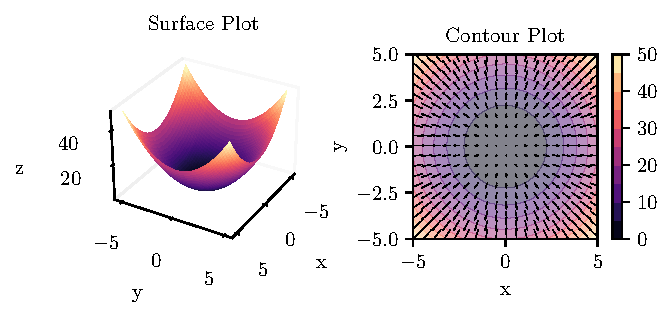
\includegraphics[scale=0.9]{../figures/mml/contour-x_squared_plus_y_squared_quiver-with-gradient.pdf}
	
	


\pause Gradient denotes the direction of steepest ascent or the direction in which there is a maximum increase in f(x,y) \\
\pause $\nabla f(x, y) = \begin{bmatrix}
\frac{\partial f(x, y)}{\partial x}\\
\frac{\partial f(x, y)}{\partial y}
\end{bmatrix} = \begin{bmatrix} 2x\\2y
\end{bmatrix}$



\end{frame}

  \section{Introduction}

  \begin{frame}{Optimization algorithms}
    \begin{itemize}
        \item We often want to minimize/maximize a function
        \item We wanted to minimize the cost function:
        \begin{equation}
            f(\theta) = (y-X\theta)^T(y-X\theta)
        \end{equation}
        \item Note, here $\theta$ is the parameter vector
        \end{itemize}   
  \end{frame}

  \begin{frame}{Optimization algorithms}
    \begin{itemize}
        \item In general, we have following components:
        \item Maximize or Minimize a function subject to some constraints
        \item Today, we will focus on unconstrained optimization (no constraints)
        \item We will focus on minimization
        \item Goal: 
        \begin{equation}
            \theta^* = \underset{\theta}{\arg\min}  f(\theta)
        \end{equation}
    \end{itemize}
    
  \end{frame}
  
\begin{frame}{Introduction}
    \begin{itemize}
    \item Gradient descent is an optimization algorithm
    \item It is used to find the minimum of a function in unconstrained settings
    \item It is an iterative algorithm
    \item It is a first order optimization algorithm
    \item It is a local search algorithm/greedy
    \end{itemize}
\end{frame}



\begin{frame}{Gradient Descent Algorithm} 
    \begin{enumerate}
        \item Initialize $\theta$ to some random value
        \item Compute the gradient of the cost function at $\theta$, $\nabla f(\theta)$
        \item For Iteration $i$ ($i = 1,2,\ldots$) or until convergence:
        \begin{itemize}
            \item $\theta_{i} \gets   \theta_{i-1} - \alpha \nabla f(\theta_{i-1})$
        \end{itemize}
    \end{enumerate}
    
\end{frame}
    

  
\section{Taylor's Series}
\begin{frame}{Taylor's Series}
    \begin{itemize}
        \item Taylor's series is a way to approximate a function $f(x)$ around a point $x_0$ using a polynomial
        \item The polynomial is given by
        \begin{equation}
            f(x) = f(x_0) + \frac{f'(x_0)}{1!}(x-x_0) + \frac{f''(x_0)}{2!}(x-x_0)^2 + \ldots
        \end{equation}
        \item The vector form of the above equation is given by:
        \begin{equation}
            f(\vec{x}) = f(\vec{x_0}) + \nabla f(\vec{x_0})^T(\vec{x}-\vec{x_0}) + \frac{1}{2}(\vec{x}-\vec{x_0})^T\nabla^2 f(\vec{x_0})(\vec{x}-\vec{x_0}) + \ldots
        \end{equation}
        \item where $\nabla^2 f(\vec{x_0})$ is the Hessian matrix and $\nabla f(\vec{x_0})$ is the gradient vector
    \end{itemize}
\end{frame}

    \begin{frame}{Taylor's Series}
        \begin{itemize}
            \item Let us consider $f(x) = \cos(x)$ and $x_0 = 0$
            \item Then, we have:
            \item $f(x_0) = \cos(0) = 1$
            \item $f'(x_0) = -\sin(0) = 0$
            \item $f''(x_0) = -\cos(0) = -1$
            \item We can write the second order Taylor's series as:
            \item $f(x) = 1 + 0(x-0) + \frac{-1}{2!}(x-0)^2 = 1 - \frac{x^2}{2}$
        \end{itemize}
        
    \end{frame}

    
    \begin{frame}{Taylor's series}
        \begin{itemize}
            \item Let us consider another example: $f(x) = x^2 + 2$ and $x_0 = 2$
            \item Question: How does the first order Taylor's series approximation look like?
            \item First order Taylor's series approximation is given by:
            \item $f(x) = f(x_0) + f'(x_0)(x-x_0) = 6 + 4(x-2) = 4x - 2$
        \end{itemize}
        
    \end{frame}



  \begin{frame}{Taylor's Series (Alternative form)}
    \begin{itemize}
    \item We have:
        \begin{equation}
            f(x) = f(x_0) + \frac{f'(x_0)}{1!}(x-x_0) + \frac{f''(x_0)}{2!}(x-x_0)^2 + \ldots
        \end{equation}
    \item Let us consider $x = x_0 + \Delta x$ where $\Delta x$ is a small quantity
    \item Then, we have:
    \begin{equation}
        f(x_0 + \Delta x) = f(x_0) + \frac{f'(x_0)}{1!}\Delta x + \frac{f''(x_0)}{2!}\Delta x^2 + \ldots
    \end{equation} 
    \item Let us assume $\Delta x$ is small enough such that $\Delta x^2$ and higher order terms can be ignored
    \item Then, we have:
    $f(x_0 + \Delta x) \approx f(x_0) + \frac{f'(x_0)}{1!}\Delta x$
    \end{itemize}


	

	
  \end{frame}

  \begin{frame}{Taylor's Series  to Gradient Descent}
    \begin{itemize}
    \item Then, we have:
    $f(x_0 + \Delta x) \approx f(x_0) + \frac{f'(x_0)}{1!}\Delta x$
    \item Or, in vector form:
    $f(\vec{x_0} + \Delta \vec{x}) \approx f(\vec{x_0}) + \nabla f(\vec{x_0})^T\Delta \vec{x}$
    \item Goal: Find $\Delta \vec{x}$ such that $f(\vec{x_0} + \Delta \vec{x})$ is minimized
    \item This is equivalent to minimizing $f(\vec{x_0}) + \nabla f(\vec{x_0})^T\Delta \vec{x}$
    \item This happens when vectors $\nabla f(\vec{x_0})$ and $\Delta \vec{x}$ are at phase angle of $180^{\circ}$
    \item This happens when $\Delta \vec{x} = -\alpha \nabla f(\vec{x_0})$ where $\alpha$ is a scalar
    \item This is the gradient descent algorithm: $\vec{x_1} = \vec{x_0} - \alpha \nabla f(\vec{x_0})$
\end{itemize}
  \end{frame}

  \begin{frame}{Effect of learning rate}
  \end{frame}

  \section{Gradient Descent for linear regression}
  \begin{frame}{Some commonly confused terms}

    \begin{itemize}[<+->]
        \item \textbf{Loss function} is usually a function defined on a data point, prediction and label, and measures the penalty. 
        \item square loss \(l\left(f\left(x_{i} | \theta\right), y_{i}\right)=\left(f\left(x_{i} | \theta\right)-y_{i}\right)^{2},\) used in linear regression
        \item \textbf{Cost function} is usually more general. It might be a sum of loss functions over your training set plus some model complexity penalty (regularization). For example:
        \item Mean Squared Error \(M S E(\theta)=\frac{1}{N} \sum_{i=1}^{N}\left(f\left(x_{i} | \theta\right)-y_{i}\right)^{2}\)
        \item \textbf{Objective function} is the most general term for any function that you optimize during training.
    \end{itemize}
    
    \end{frame}

    \begin{frame}{Gradient Descent : Example}
        Learn $y = \theta_0 + \theta_1 x$ on following dataset, using gradient descent where initially $(\theta_0, \theta_1) = (4,0)$ and step-size, $\alpha  = 0.1$, for 2 iterations. 
        \begin{table}[]
            \centering
            \label{tab:my-table}
            \begin{tabular}{|c|c|}
                \hline
                \textbf{x} & \textbf{y} \\ \hline
                1 & 1 \\ \hline
                2 & 2 \\ \hline
                3 & 3 \\ \hline
            \end{tabular}
        \end{table}
        \end{frame}
        
        

    \begin{frame}{Gradient Descent : Example}
        Our predictor, $\hat{y} = \theta_0 + \theta_1x$\\
        \vspace{1cm}
        Error for $i^{th}$ datapoint, $\epsilon_i = y_i - \hat{y_i}$\\
        $\epsilon_1 = 1 - \theta_0 - \theta_1$ \\
        $\epsilon_2 = 2 - \theta_0 - 2\theta_1$ \\
        $\epsilon_3 = 3 - \theta_0 - 3\theta_1$ \\
        
        \vspace{1cm}
        MSE = $\dfrac{\epsilon_1^2 + \epsilon_2^2 + \epsilon_3^2}{3}$ = $\dfrac{14 + 3\theta_0^2 + 14\theta_1^2 -12\theta_0 - 28\theta_1 + 12\theta_0\theta_1}{3}$\\
        \end{frame}
        
            \begin{frame}{Difference between SSE and MSE}
        
        
        
        \begin{equation*}
        \sum \epsilon_{i}^{2} \textit{ increases as the number of examples increase}
        \end{equation*}
        
        So, we use MSE
        
        \begin{equation*}
        \textit{MSE} = \frac{1}{n} \sum \epsilon_{i}^{2}
        \end{equation*}
        
        Here $n$ denotes the number of samples
        
        
        
        \end{frame}
  

 
\end{document}